 \documentclass{article}
\usepackage{verbatim}
\usepackage[utf8]{inputenc}
\usepackage{graphicx}
\usepackage{float}
\usepackage[margin=1in]{geometry}
\usepackage{enumitem}
\title{S function}
\date{}

\begin{document}
\maketitle
S functions are a way to add C/C++ or any other language function to a Simulink model. These function are used to create custom blocks for very specific tasks. Most popular S function are built using the C, C++ and FORTRAN. A main driving factor for S function is that it can be saved and is transferable to another model simulation.
\subsection{There are two ways to write S-function in Simulink.}
\begin{enumerate}
    \item \textbf{Legacy\_Code Method of S-Function}: This method there is less control on the simulation but it is computationally very efficient and more versatile. There is no need for major changes in the pre-existing C/C++ code, here \textbf{legacy\_code} creates C\C++ code which can be used in both Matlab and Simulink. This method is preferred for hardware simulations.




    \item \textbf{Level 2 S- function}: Here the C program is written in the "wrapper file". There is more control of the S-function because simulation structure SimStruct is accessible in this method. (SimStruct is simulation data storing structure where parameters control all simulations in Sumlink model eg. simulation time, input parameters, output data type etc) . In Level-2 S function, Matlab provides processing functions which controls the SimStruct. Matlab also provides a GUI based approach for this called S-function Builder. S-function Builder method acts a GUI for the level-2 method. 



\end{enumerate}
\subsection{Standard Variable Nomenclature}
Following nomenclature must be used while declaring input, output or parameters in the S function. These variable names remains constant for all type of S functions. Note that pointers can be used in the C/C++ functions, but should be declared like an array in S function declaration. Without the nomenclature the legacy code does not compile C/C++ code.
\begin{enumerate}
    \item Input Variables
    \begin{enumerate}
        \item For N input variables, syntax format is u1.....un.
        \item For a variable array of dimension m1,m2.,syntax format is u1[m1],u2[m2].
    \end{enumerate}
    \item Output variable
    \begin{enumerate}
        \item For N output variables, syntax format is y1.....yn.
        \item For a variable array of dimension m1,m2., syntax format is  y1[m1],y2[m2].
    \end{enumerate}
    \item Parameters
    \begin{enumerate}
        \item For N parameters variables, syntax format is p1.....pn.
        \item For a variable array of dimension m1,m2., syntax format is  p1[m1],p2[m2].
    \end{enumerate}
\end{enumerate}
\subsection{General flow of the S function}
The S function we write in any language should also follow this flow of operation. To solve a differential equation integration protocol can be coded in S function eg, Euler and RK4 . But in Level 2 S function Matlab also provide an integration function, which will execute the integration type set in the Simulink properties. In other words, for the systems involving differential equations, we can either 
\begin{itemize}
    \item Provide our own numerical integration algorithm.
    \item Use Matlab/Simulink integration function and choose it in the simstruct property.
\end{itemize}
\subsubsection*{Flow of S function operation:}
\begin{enumerate}[label=Step \arabic*]
    \item First step is initialization step, here the Parameters, input and output variable size allocation is done.\\ In this step general syntax of the function and methods called is also verified.
    \item Next is the simulation loop, this is only executed if there are simulation time depended functions in the code. The simulation loop is independent of the initialization stage.
    \begin{enumerate}
        \item Calculate the output of the functions for the first time step.  
        \item If there is any derivative function execute this function and update the the output.
        To use this pass the states to the function \textbf{differentiate()} in level 2-function and in C mex function use mdl\_derivative library.
        \begin{verbatim}
        #define MDL_DERIVATIVES
        void mdlDerivatives(SimStruct *S)
        \end{verbatim}
    \end{enumerate}
    \item Repeat the Step 2 loop until simulation time is complete
\end{enumerate}
\begin{figure}[H]
    \centering
    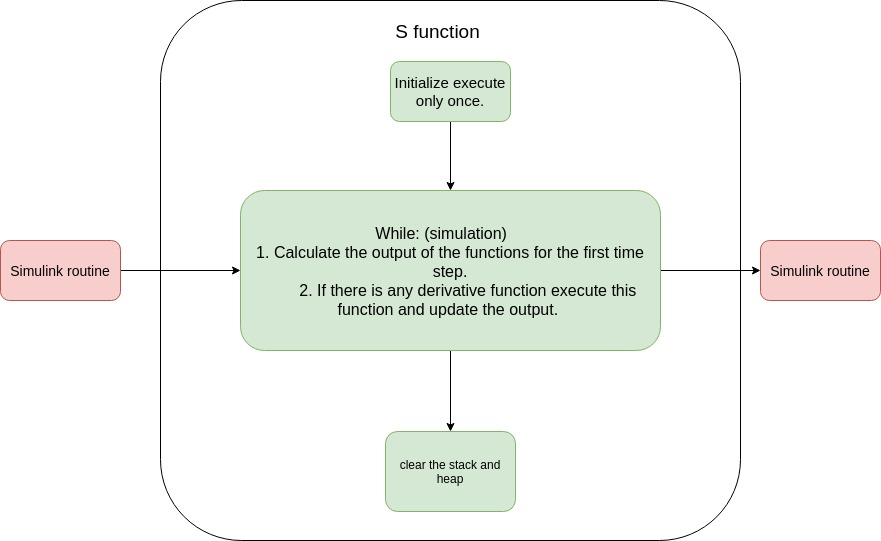
\includegraphics[width=\textwidth]{cep.jpg}
    \caption{Flow chart of the S function.}
    \label{fig:my_label}
\end{figure}
\subsection{Prerequisite }
Common C-compilers are as follows:
\begin{enumerate}
    \item \textbf{Windows} C++ compiler mingw can be downloaded using the Add-On Manager in the Matlab environment.
    If using other MinGW installation other than Matlab i.e. Visual Studio, Codeblocks , you have set to the environment path to the Matlab, using the command.
    \begin{verbatim}
        setenv('MW_MINGW64_LOC',location of the file)
    \end{verbatim}
    \item \textbf{Linux / Mac OS} GNU g++ Compiler installed in the system already.
\end{enumerate}
To test the installation of the C compiler, type following command in the command window

\begin{verbatim}
   >> mex -setup
\end{verbatim}
There is a build in Matlab example to test the working and and to know the working of the files called as y prime. 
We will use this file to test the working of the function before we write the custom function.
\begin{verbatim}
copyfile(fullfile(matlabroot,'extern','examples','mex','yprime.c'),'.','f')

%this will get the file to the current directory

>>mex yprime.c

%this command will be build the executable file using the compiler
%to test mex file in matlab

>>T=1;
>>Y=1:4;

>>yprime(T,Y)
\end{verbatim}
the output file should look like the following file
\begin{figure}[h]
\centering
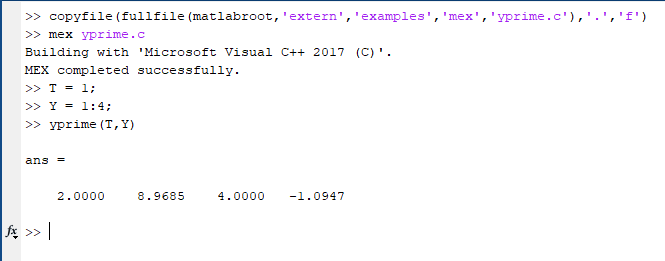
\includegraphics[width=0.5\textwidth]{Capture1.PNG}
\caption{there must be a file with extension *.mexw64 along with the *.c file, This shows that compiler is working properly in the matlab.}
\end{figure}
\begin{figure}[H]
    \centering
    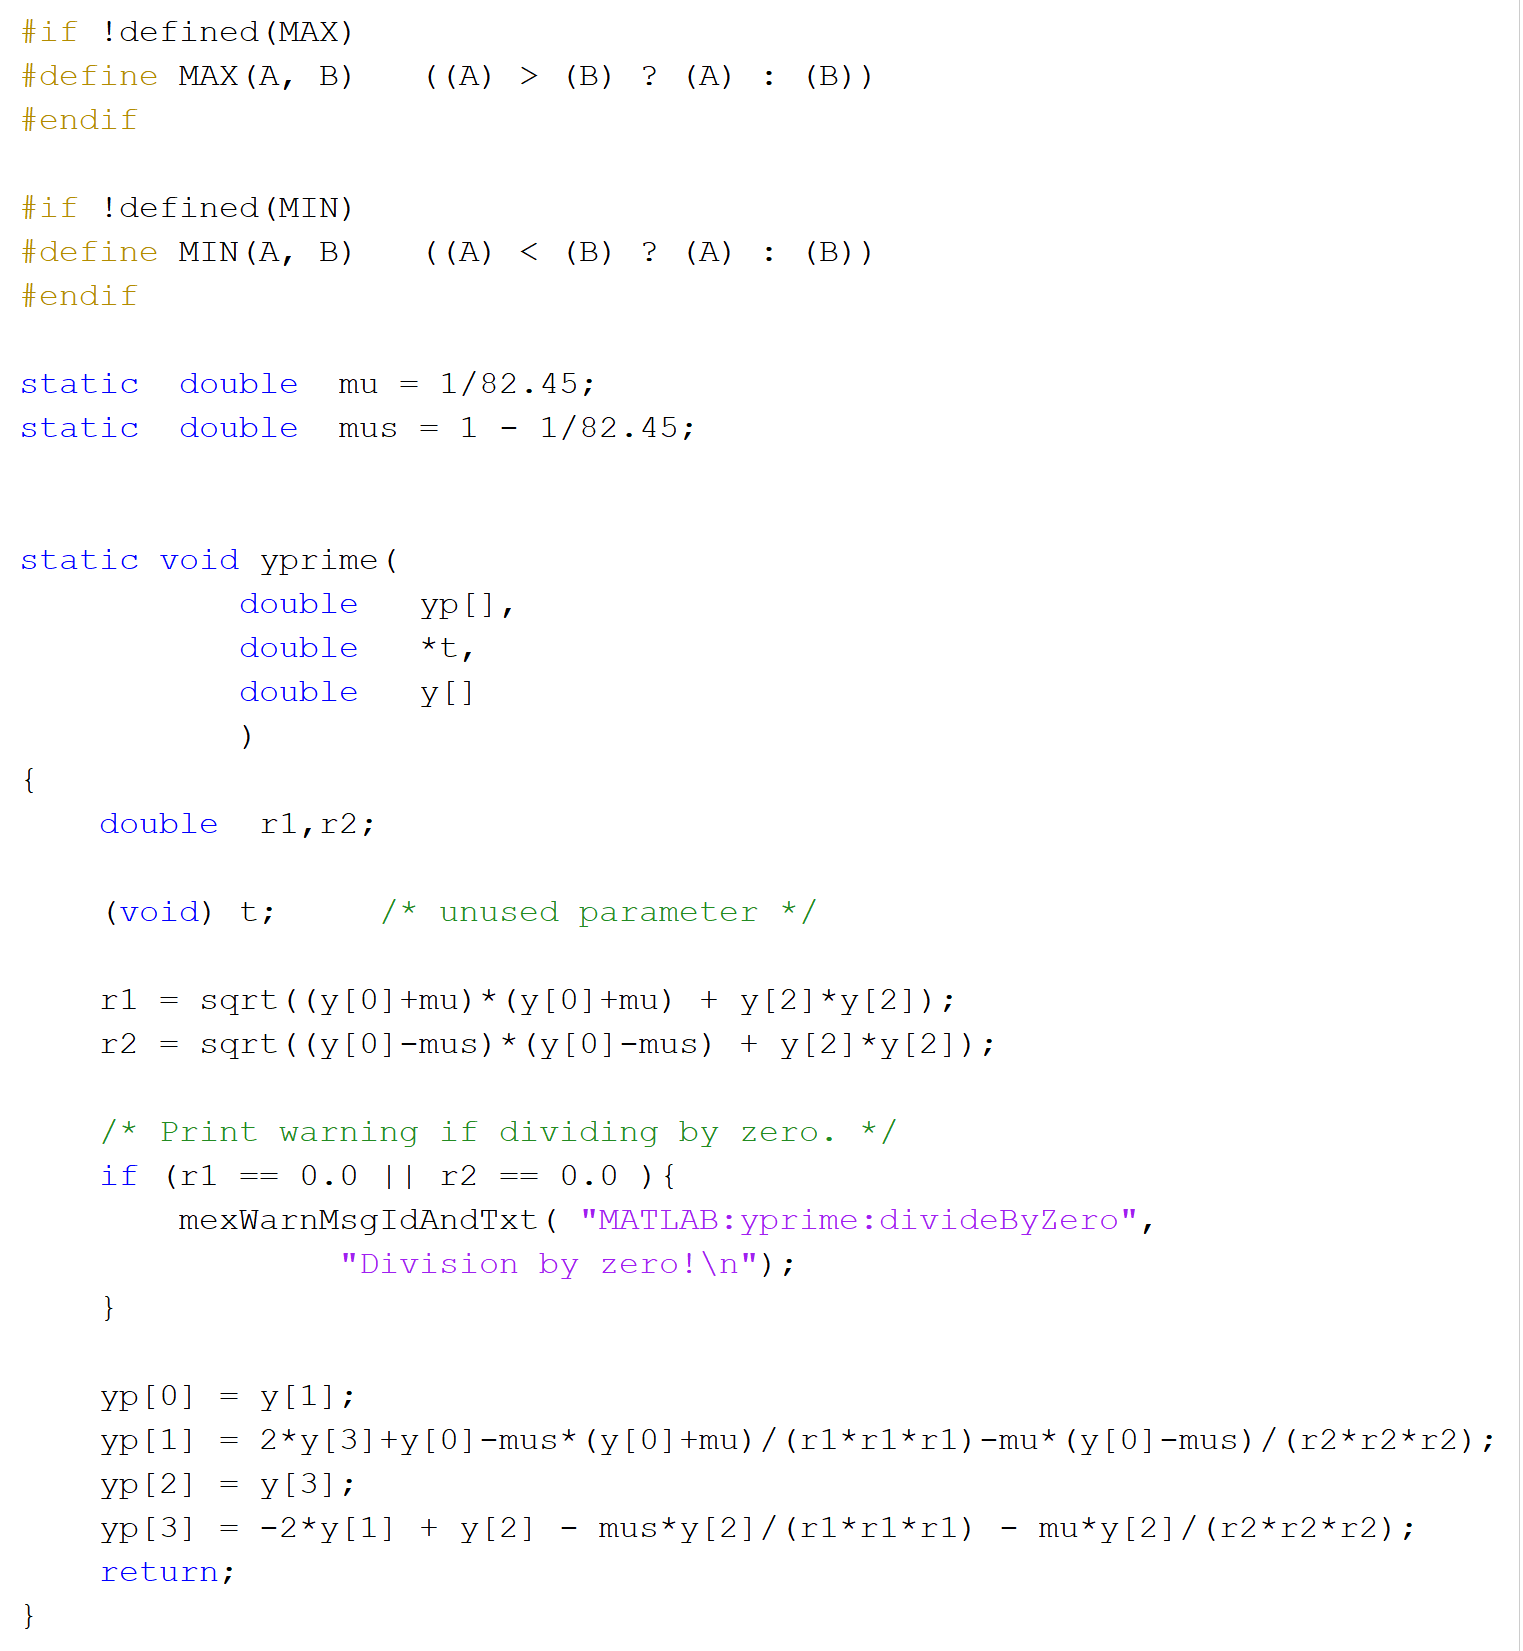
\includegraphics[width=\textwidth]{Capture.PNG}
    \caption{Snap shot of source code yprime.c}
    \label{fig:my_label}
\end{figure}
\section{Legacy\_code method of S-Function}
S function are the Simulink block which enables the use of the c and c++ files i.e \textbf{*.c}, \textbf{*.cpp} and supporting header files \textbf{*.h}, \textbf{*.hpp}
\subsection{S Function Development Using Legacy Code}
\begin{enumerate}
    \item Develop a C/C++ code for the desired operation, make sure there is no \textbf{main()} function in the project. Also write the .h file for the function in C++ code.
    \item Initialize a legacy\_code development structure and declare the \textbf{Parameters}, \textbf{Inputs} and \textbf{Outputs} of the S function. Also add the parent functions (Output and Input/Initialization functions, which are C/C++ functions,to receive or output values to the simulink.), \textbf{note that parent functions declaration syntax is in m file and not C++.} 
    \item Build, compile legacy\_code structure, which results is a wrapper .c function and .mex file.
    \item Open a new Simulink workspace, add the S function block to the workspace. Rename the block in the name of the function which was created, enter the parameters value in the dialog box of the properties section.
    \item Now the S-function is ready for the use. These function are reusable in other simulink models, if .c and .mex files are transferred.
\end{enumerate}

\subsection{Example: Step function}
Now lets do the custom step saturation function which give output 1 if the any value more than 5 is given in Simulink.
\subsubsection{ Making mex file }
\begin{enumerate}
    \item Create two C++ file using texteditor and save in the same workspace
    \begin{verbatim}
    
        \* file my_step.c *\
    
        #include "my_step.h"
    
        double step(double a)
        {
            double b;
            if (a>5){
                b = 1;
            }
            else{
                b=0;
            }
            return(b);
    
        }

        %%
        \* file my_step.h *\
        #ifndef MY_STEP_H_INCLUDED
        #define MY_STEP_H_INCLUDED
        
        double step(double a);
        
        #endif
    \end{verbatim}
    
    \item Create a structure that will store the properties of the .c file. using the command
    \begin{verbatim}
        struc = legacy_code('initialize')
    \end{verbatim}
    This is will create a structure with fields:
    \begin{verbatim}
        struc = 

  struct with fields:

                  SFunctionName: ''
    InitializeConditionsFcnSpec: ''
                  OutputFcnSpec: ''
                   StartFcnSpec: ''
               TerminateFcnSpec: ''
                    HeaderFiles: {}
                    SourceFiles: {}
                   HostLibFiles: {}
                 TargetLibFiles: {}
                       IncPaths: {}
                       SrcPaths: {}
                       LibPaths: {}
                     SampleTime: 'inherited'
                        Options: [1 x 1 struct]
    \end{verbatim}
     Now we have to change the various attributes to the S-Function like name, sourcefile, headerfile etc
    \begin{verbatim}
        struc.SFunctionName = 'my_step_block'
        
        %This is the name of the S Function which will be created
    \end{verbatim}
     Output function: Output function is a wrapper function which take the Input from the Simulink/ Matlab and compute output from the C++ code. Here nomenclature used in the output function:
    \begin{enumerate}
        \item \textbf{$y1,y2,y3.....yn$} are used for different outputs.
        \item \textbf{$u1,u2,u3.....un$} are used for different input ports.
        \item Array and pointers inputs and outputs should be called as \textbf{ $y1[1...n]$ and $x1[1....n]$ }
        \item \textbf{$p1,p2,p3.....pn$} are used for different parameters.
    \end{enumerate}
    In this case there is only one Input port $u1$ and one output port $y1$
    \begin{verbatim}
        struc.OutputFcnSpec = 'double y1 = step(double u1)'
    \end{verbatim}
     Populate the structure with the source file and the header file. To add multiple .h and .c use the same struct and declare 
    \begin{verbatim}
        struc.HeaderFiles = {'my_step.h'}
        struc.SourceFiles={'my_step.c'}
    \end{verbatim}
    
    Now the final struc will look like the following.
    \begin{verbatim}
        struc = 

  struct with fields:

                  SFunctionName: 'my_step_block'
    InitializeConditionsFcnSpec: ''
                  OutputFcnSpec: 'double y1 = step(double u1)'
                   StartFcnSpec: ''
               TerminateFcnSpec: ''
                    HeaderFiles: {'my_step.h'}
                    SourceFiles: {'my_step.c'}
                   HostLibFiles: {}
                 TargetLibFiles: {}
                       IncPaths: {}
                       SrcPaths: {}
                       LibPaths: {}
                     SampleTime: 'inherited'
                        Options: [1 x 1 struct]
    \end{verbatim}
\item Create the .c and compile this code using the legacy\_code compile statement as follows
\begin{verbatim}
    legacy_code('sfcn_cmex_generate',struc)
    legacy_code('compile',struc)
\end{verbatim}
Matlab will create two files in the workspace a .mex file and a .c file, these two files are used to develop S-function in simulink and also these files are transferable to other directory.

\item Loading an S function in Simulink model
\begin{enumerate}
    \item Add S function block from simulink library browser.
    \item Rename the block from the default name - \textbf{system} to the name \textbf{name of the block}
    \item Output should look like the following figure \ref{fig:fig20}
\begin{figure}[h]
\centering
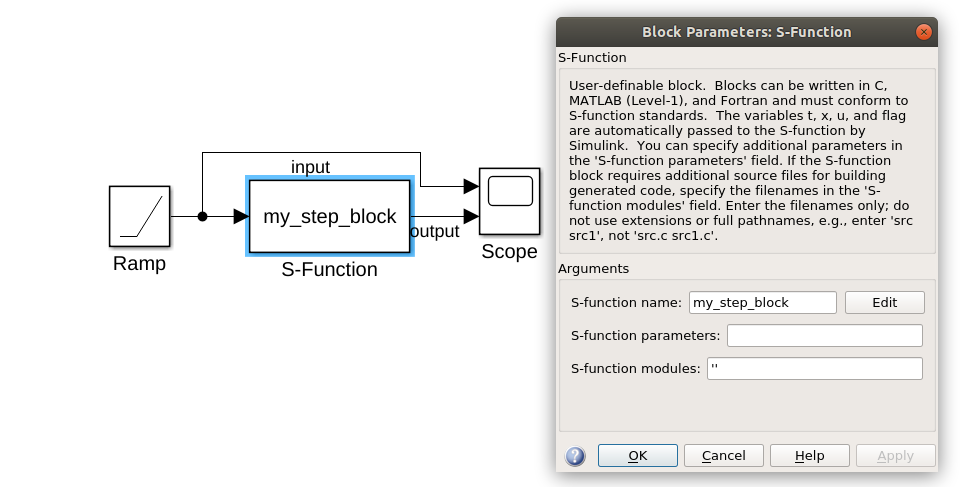
\includegraphics[width=\textwidth]{fig12.png}
\caption{Add and configure an S-function block in a simulink model. The name of the block should be same as the name given in the legacy_code and .mex file should in the working directory}
\end{figure}
\end{enumerate}
Now add the function with the input test signal and run the simulation.
The results should be as follows:
\begin{figure}[H]
\centering
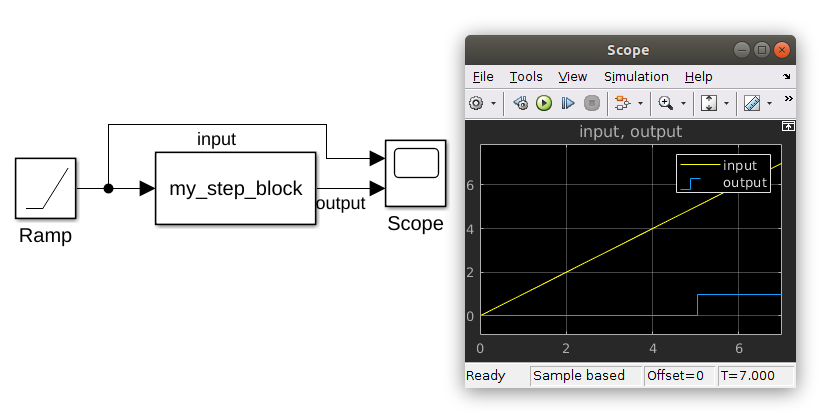
\includegraphics[width=\textwidth]{fig11.png}
\caption{Simulation output of the block}
\label{fig:fig20}
\end{figure}
\end{enumerate}
\subsection{Example: Spring mass force system using PID controller}
\begin{figure}[H]
    \centering
    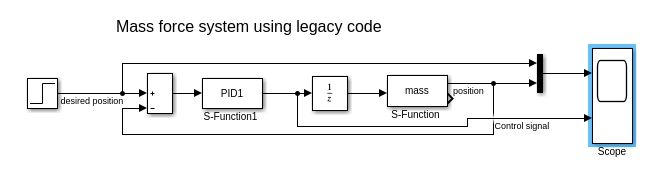
\includegraphics[width=\textwidth]{Selection_002.jpg}}
    \caption{Mass force system built using S-functions}
    \label{fig:modellega}
\end{figure}
\begin{enumerate}
    \item C++ code for the mass force dynamics.
    \begin{verbatim}
    #include "math.h"
    #include "massc.h"
    void mass(double u, double K, double C,double M, double delta_t, double *y1, double *y2)
    {
    // u - input , K,C,t - parameters, y1 and y2 are pointers for the output.
    // U - control input
    // K, C are spring constant and damping
    // t - euler time step
    //x_dot is the velocity and acceleration
    // new_x is the updated velcoty and distance
    double x_dot[2];
    static double new_x[2] = {0.0,0.0};
    x_dot[0] = new_x[1];
    x_dot[1] = (1/M) * (u - K * new_x[0] - C * new_x[1]);
    new_x[0] = euler(x_dot[0],new_x[0],delta_t);
    new_x[1] = euler(x_dot[1],new_x[1],delta_t);
    *y1 = new_x[0];
    *y2 = new_x[1];
    }
    
    
    
    double euler(double y,double x,double delta_t)
    {
    double z = y * delta_t + x;
    return z;
    }
    \end{verbatim}
    H File
    \begin{verbatim}
    #ifndef MASSC
    #define MASSC
    double euler(double y,double x,double delta_t);
    void mass(double u, double K, double C,double M, double delta_t, double *y1, double *y2);
    #endif
    \end{verbatim}
    For the this C++ code the parameters are K,C,M and delay time ( Euler time and step ). Input is u and output pointer are y1 and y2. The code is given below.Here, Euler method of differentiation is used and other more complex methods can be used.\\
    \item C++ code for the PID control. 
    \begin{verbatim}
    %%%% file PIDC.cpp
    #include "PIDC.h"
    #include "math.h"
    double pid (double error ,double Kp ,double Ki,double Kd)
    {
    static double previous_error = 0;
    static double error_integral = 0.0;
    // error - input; P,I,D paramters
    double P_out,I_out,D_out,PIDOut;
    P_out = error * Kp;
    error_integral = error_integral + error;
    I_out = error_integral * Ki;
    D_out = (error-previous_error) * Kd;
    PIDOut = P_out + I_out + D_out;
    previous_error = error;
    return PIDOut;
    }
    \end{verbatim}
    H file
    \begin{verbatim}
        %%%% file PIDC.h
    #ifndef PIDC
    #define PIDC
    #include "iostream"
    double pid (double error ,double Kp ,double Ki,double Kd);
    #endif
    \end{verbatim}
    For the this C++ code the parameters are P,I and D. Input is error and output is out.
    
    \item Build and compile the Mass and PID controller code using the legacy\_code. 
    The following code is used to create the mex code for the PID and mass block.
    \begin{verbatim}
massstruct = legacy_code('initialize');
massstruct.SFunctionName = 'mass';
massstruct.SourceFiles = {'massc.cpp'};
massstruct.HeaderFiles = {'massc.h'};
massstruct.OutputFcnSpec =  'void mass(double u1, double p1, double p2, double p3, double p4, double y1[1], double y2[1])';
pidstruct  = legacy_code('initialize');
pidstruct.SFunctionName = 'PID1';
pidstruct.SourceFiles = {'PIDC.cpp'};
pidstruct.HeaderFiles={'PIDC.h'};
pidstruct.OutputFcnSpec = 'double y1 = pid(double u1, double p1, double p2, double p3)';
legacy_code('sfcn_cmex_generate',massstruct);
legacy_code('compile',massstruct);
legacy_code('sfcn_cmex_generate',pidstruct);
legacy_code('compile',pidstruct);
    \end{verbatim}
    \item In Simulink, add 2 S-function blocks to the workspace and in the system change the block parameters as the figure shown below\\
    Note: Parameters order is declared in cpp file and the legacy\_code struct as indicated below.
    \\Mass force dynamics parameters order of declaration is as follows.
    \begin{verbatim}
void mass(double u, double K, double C,double M, double delta_t, double *y1, double *y2);
massstruct.OutputFcnSpec =  'void mass(double u1, double p1, double p2, double p3, double p4, double y1[1], double y2[1])';
// Here parameters are K is p1, C is p2, M is p3, delta_t is p4.
    \end{verbatim}
    
    PID controller parameters order of decleration are as follows.
    \begin{verbatim}
double pid (double error ,double Kp ,double Ki,double Kd);
pidstruct.OutputFcnSpec = 'double y1 = pid(double u1, double p1, double p2, double p3)';
// Here parameters are Kp is p1, Ki is p2, Kd is p3.
    \end{verbatim}
    Based on these order the parameters are populated. 
    \begin{figure}[H]
        \centering
        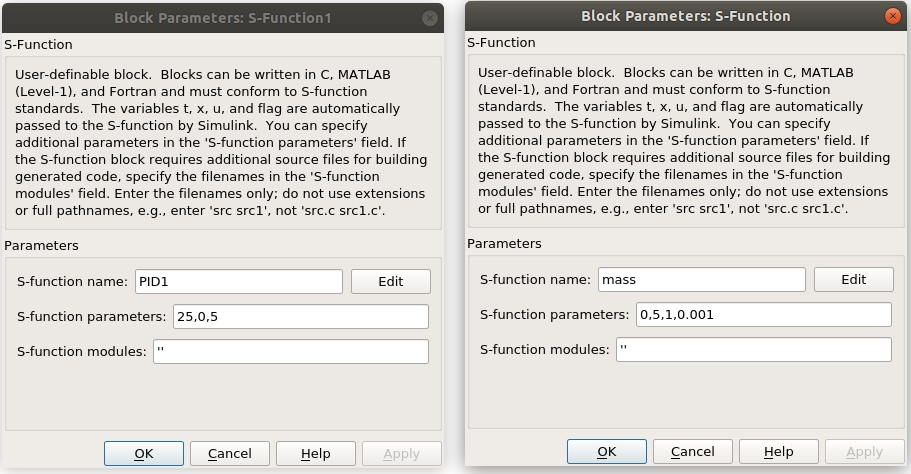
\includegraphics[width=\textwidth]{Selection_011.jpg}
        \caption{block parameters for the S-function block.}
    \end{figure}
    \item Construct the Simulink model as show in the fig \ref{fig:fig4}. Since Custom numerical integration is provided and time step of that is 0.001 add a unit delay block with identical delay. Note is the unit delay block is not added result will go infinity and simulink is display an error.
    \begin{figure}[H]
        \centering
        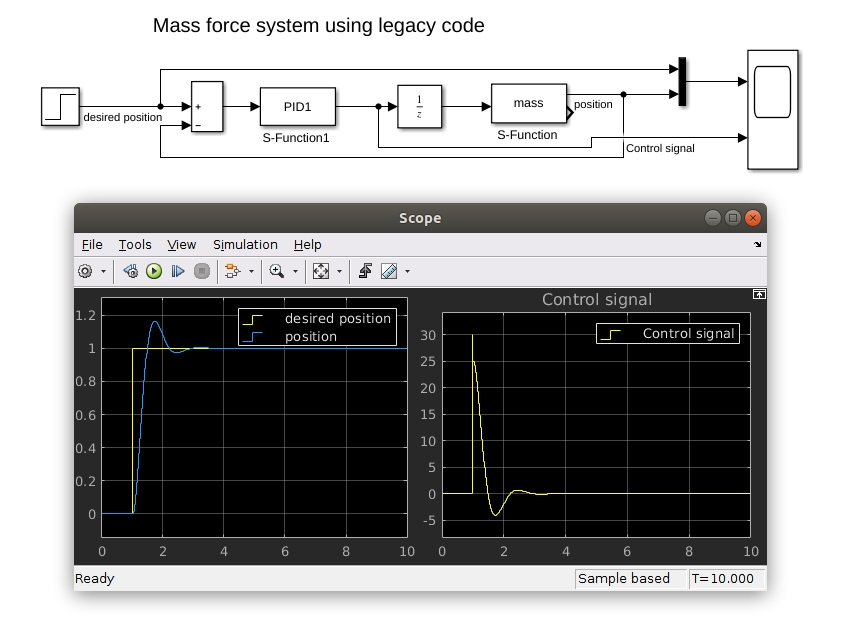
\includegraphics[width=1.1\textwidth]{Selection_012.jpg}
        \caption{Results.}
        \label{fig:fig4}
    \end{figure}
\end{enumerate}

\section{S Function Builder}
This is a built in Simulink block which provides a GUI for \textbf{parameters, Input and Output} variable and its size declarations. 
\textbf{Simulink builder} not only has all the advantages of that of legacy\_code but also provides initialization parameters (states), whose value can be initialized in the beginning of code and can dynamically changed. 
\textbf{S function builder} is a GUI over the level-2 S function, So this builder will create a wrapper.c file where the c code can be changed. S function builder follows the syntax and function calling method similar to that of the level 2 s function.
\subsection{Steps for using S function  builder in simulink}
\begin{enumerate}
    \item Copy the S Function Builder from Simulink toolbox into the \textbf{Simulink model}.
    \item Double click on block to open the parameters windows as shown in the figure.
    \item Now there are 9 tabs window, where the characteristics of the S function can be changed. \\\textit{ Declaration that needs to be done in this section is in the C programming syntax and pointers can be used}
    \begin{enumerate}
        \item \textbf{Initialize:} Here the variable are discrete and continuous states are declared. These states values can be stored and used in different time step of simulation. \\
        To access discrete states we have to use, xD[0 ... 10]\\
        To access continuous states we have to use xC[0 ... 10]\\
        Also note do not use xd use xD. 
        \item \textbf{Data properties:} In this sections we declare the input, output and parameters size and data type. Input output and parameters can be declared as array and also multiple input and output for a block can be declared here.
        \item \textbf{Libraries:} Here the header files and the source files are added. Also the functions used in the source file and not declared in the .h file should be declared in the dialog box given.
        \item \textbf{Start:} Here the states are declared and initialized. Note that this part of code will run once at the start of the simulation. 
        \item \textbf{Output:} Here the output functions are declared, the output functions are the ones which are responsible for the output y1[0],y1[0] .... y1[n] , the code or algorithm which needs to run will be called in this function. Making this main() or (parent) function and all the functions declared in the libraries section are nested functions. To access input variables enable the check mark at the bottom. Function calling the other files can be coded here.
        \item \textbf{Differentiate:} If any state needs to differentiated it will be declared here.
        \item \textbf{Update:} If states need to be update after each simulation time, then state with update condition should be declared here.
        \item \textbf{Terminate:} Here the part of code that need to run at the end of all the simulation, is declared eg. freeing up the memory in the ram etc.
        \item  \textbf{Build info:} When the S function is built, this section will provide the information of the C files which are created. 
    \end{enumerate}
    \begin{figure}[H]
        \centering
        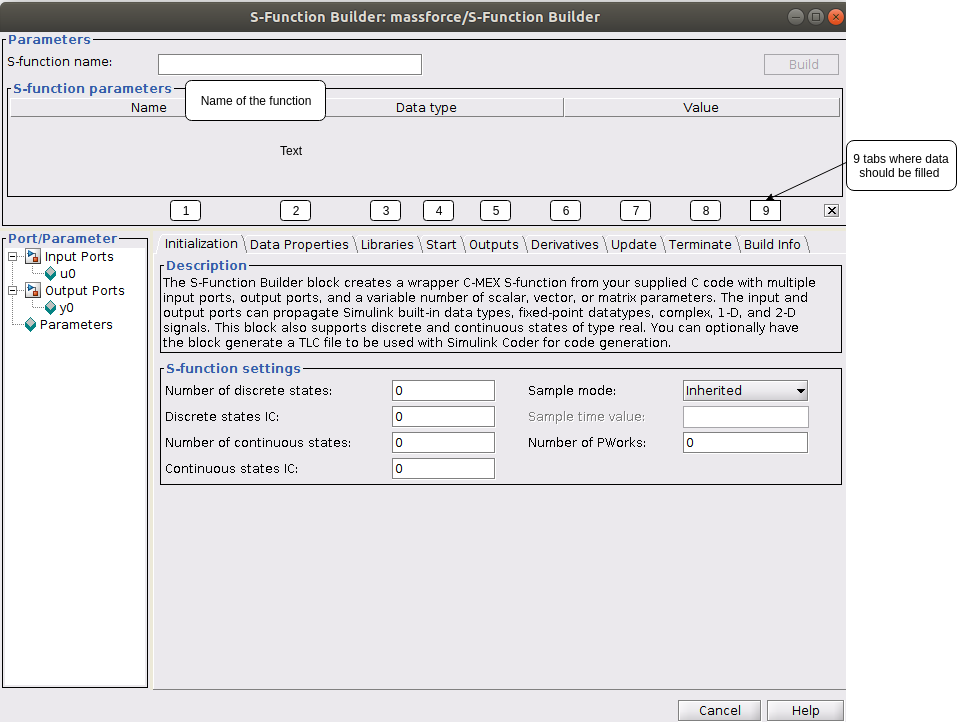
\includegraphics[width=\textwidth]{9Tabs.png}
        \caption{(9 windows where data must be populated.}
        \label{fig:my_label}
    \end{figure}
\item When S function is build, it will create\textbf{ two *.C files, one .TLC files} and \textbf{one complied S function file}. One of the C file created is a wrapper file where the function can be called, another  is complete S function code in level 2 S function format. If the properties of the function is changed in the file must be built again.
\end{enumerate}
\subsection{Example: Mass force system with PID controller}
\begin{figure}[H]
    \centering
    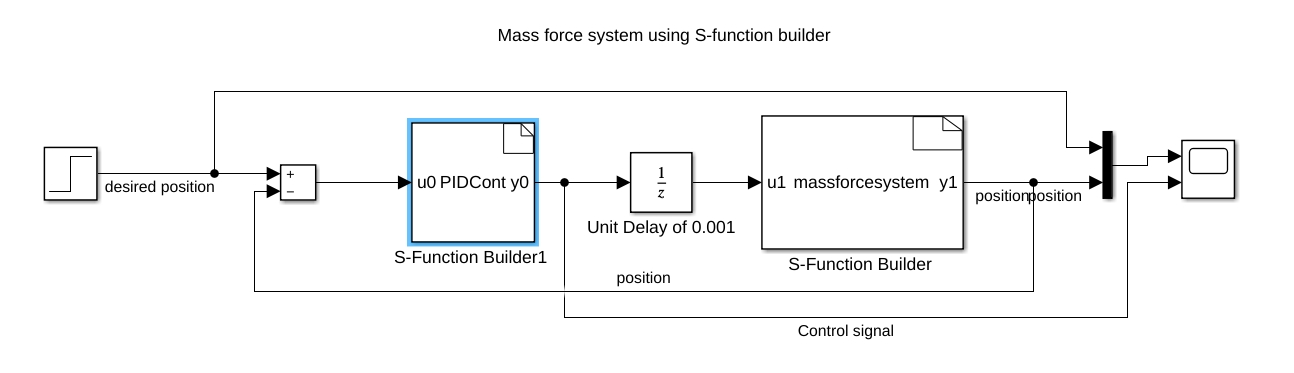
\includegraphics[width=\textwidth]{Selection_009.jpg}
    \caption{Mass force system}
    \label{fig:block_builder}
\end{figure}
\begin{enumerate}

\item \textbf{C/C++ files}
\textbf{Mass dynamics system files}

\begin{verbatim}
%%%%%%%%%%% file name massc.cpp %%%%%%%%%%%%%%%%%%%%%%%%%%%%%%%%%%
#include "math.h"
#include "massc.h"

double mass(double *delta_t ,double u1, double *K, double *C, double *M)
{   
    // u - input , K,C,t - parameters
    // U - control input
    // K, C are spring constant and damping
    // delta_t - euler time step
    //x_dot is the velocity and acceleration
    //new_x[0] in the distance
    double x_dot[2];
    static double new_x[2] = {0.0,0.0};
    // Note: All the paramters must be pointers, Input and state are variables(double),
    x_dot[1] = (1/ *M) * ( u1  - *K * new_x[0] - *C * new_x[1]);
    x_dot[0] = new_x[1];
    new_x[0] = euler(x_dot[0],new_x[0], *delta_t);
    new_x[1]  = euler(x_dot[1],new_x[1], *delta_t);
    return new_x[0];
}

double euler(double y,double x,double delta_t)
{
    double z = y * delta_t + x;
    return z;
}



%%%%%%%%%%%% file name massc.h %%%%%%%%%%%%
#ifndef MASSC
#define MASSC

double euler(double y,double x,double t);
double mass(double *delta_t, double u1, double *K, double *C, double *M);
#endif

\end{verbatim}
\textbf{PID controller files}
\begin{verbatim}
%%%%%%%% file name PIDC.cpp %%%%%%%%%%%%%%%%%
#include "PIDC.h"
#include "math.h"

double pid (double error ,double *Kp ,double *Ki,double *Kd)
{   
    // error - input P,I,D paramters
    static double previous_error = 0;
    static double error_integral = 0.0;
    // Note: all the paramters should be double variable.
    double P_out,I_out, D_out, Out;
    P_out  = error * *Kp;
    I_out =  error_integral * *Ki;
    D_out = (error-previous_error) * *Kd;
    Out = P_out +  I_out + D_out;
    //update
    previous_error = error;
    error_integral = error + error_integral;
    return Out;
} 
%%%%%%%%% file name PIDC.h %%%%%%%%%%%%%%%%%%
#ifndef PID
#define PID
#include "iostream"
double pid (double error ,double *Kp ,double *Ki,double *Kd);
#endif
\end{verbatim}
\item Load the S function builder to the Simulink workspace. Double click the function to get the properties in the GUI or also called as function builder. As shown in the fig 
\begin{figure}[H]
    \centering
    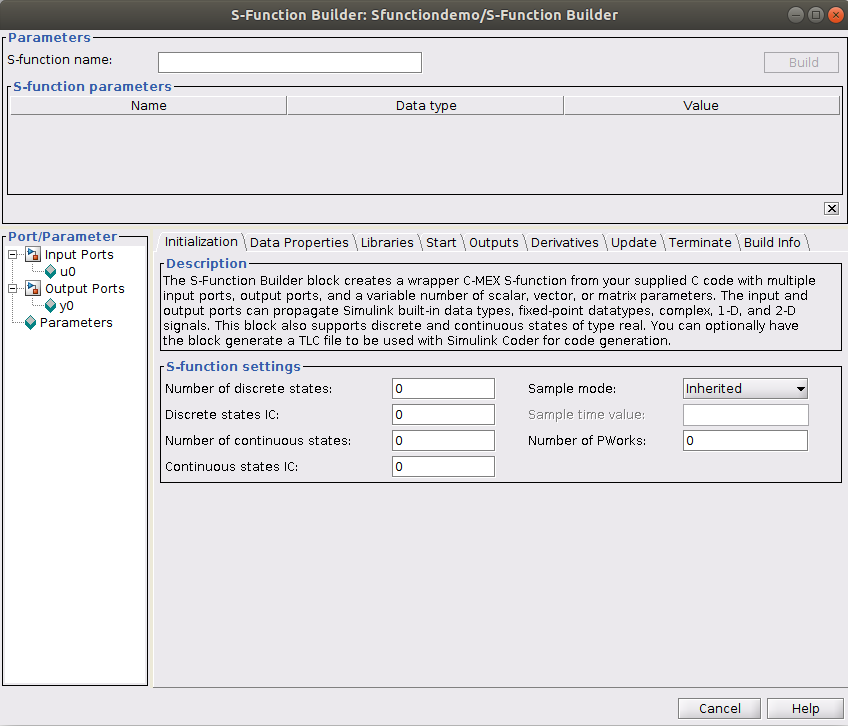
\includegraphics[width=0.8\textwidth]{Selection_008.png}
    \caption{Fill dialog box of the new block}
    \label{fig:blank}
\end{figure}
\item Name the S-funtion as \textbf{massforcesystem}
\item In the Data $Properties \to Input ports \to add\, or\, rename\, the\, port$ similarly follow the name procedure. \\ 
For the system parameters go the $Data Properties \to Parameters$
add parameters K,C,m,and delta\_t.
\item In the Libraries tab in the GUI. Add the Source file, \textbf{massc.cpp} and in the Header file \textbf{#include "massc.h"}.
\item Now in the output tab, call the function.
\begin{verbatim}
y1[0] = mass( (double*)delta_t,u1[0], (double*) K,  (double*)C,  (double*)M);
\end{verbatim}
\item In the build Info tab, check "Generation wrapper TLC". and Build the system, Now there will be a *\_wrapper.c, *.c and *.tlc file in the workdirectory. the TLC file is transferable.
\begin{figure}[H]
    \centering
    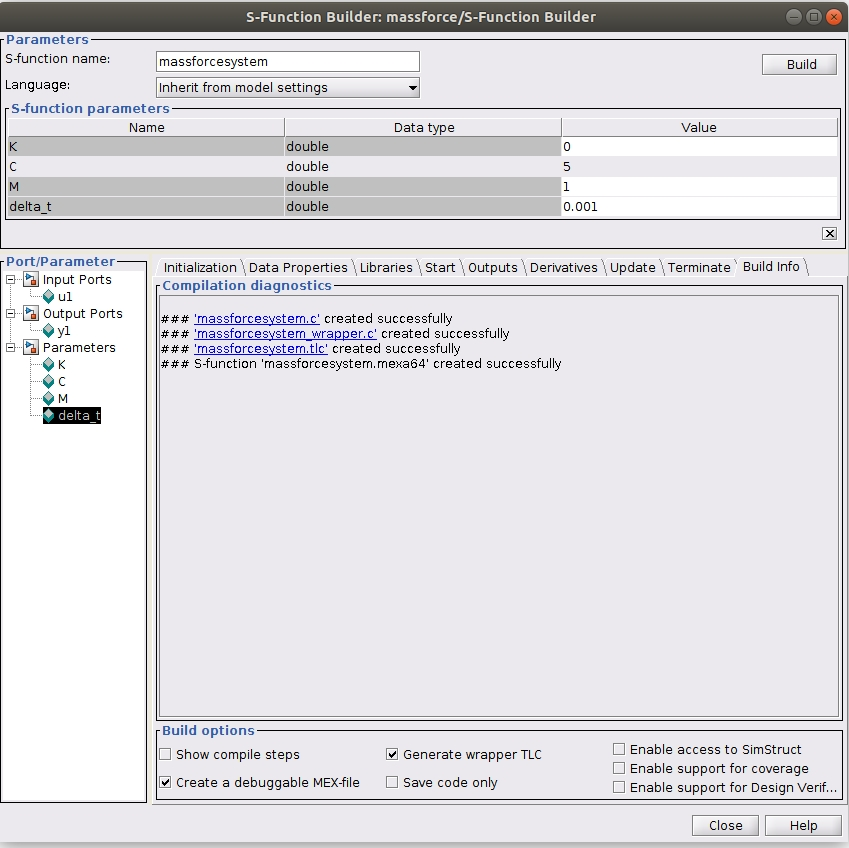
\includegraphics[width=0.8\textwidth]{Selection_014.jpg}
    \caption{Output of the dialog box after building the function.}
    \label{fig:outputmass}
\end{figure}
\item Open another S-function block in the block for PID controller.
\item In the parameters section in the "data parameters" add \textbf{P,I and D}.
\item In the header file section of libraries add \textbf{#include "PIDC.h"} and in the source file section add the \textbf{PIDC.cpp} file.
\item Build the function in the output of that function will look like fig\ref{fig:pid_builder}
\begin{figure}[H]
    \centering
    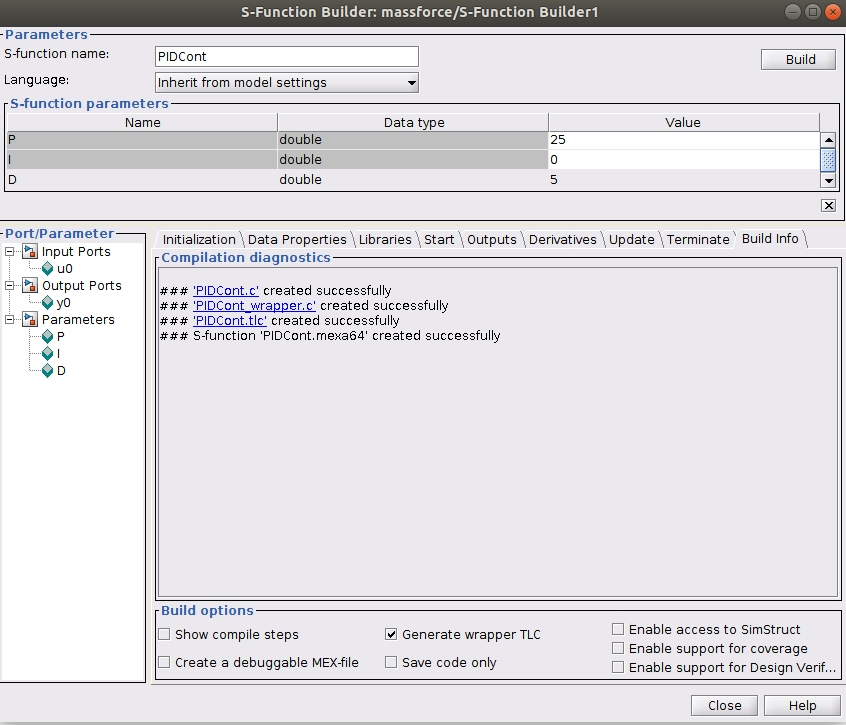
\includegraphics[width=0.8\textwidth]{Selection_015.jpg}
    \caption{Pid controller S function output.}
    \label{fig:pid_builder}
\end{figure}
\end{enumerate}
\begin{figure}[H]
    \centering
    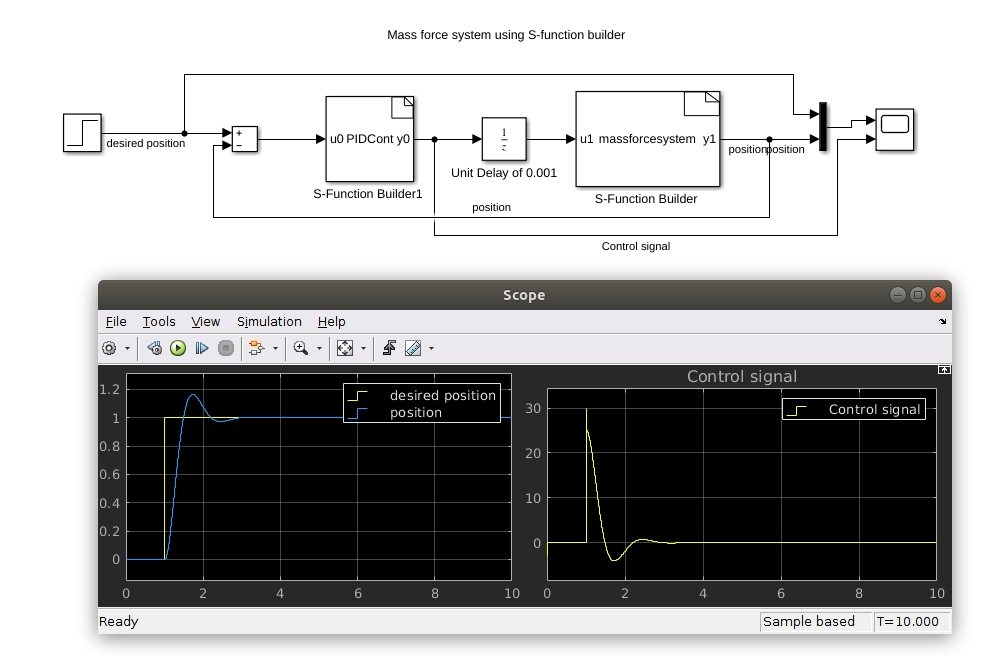
\includegraphics[width=0.\textwidth]{Selection_013.jpg}
    \caption{Output of the mass force system with PID controller}
    \label{fig:output_builder}
\end{figure}
\subsection*{Pictorial example of data populated S function builder.}
\begin{figure}[H]
    \centering
    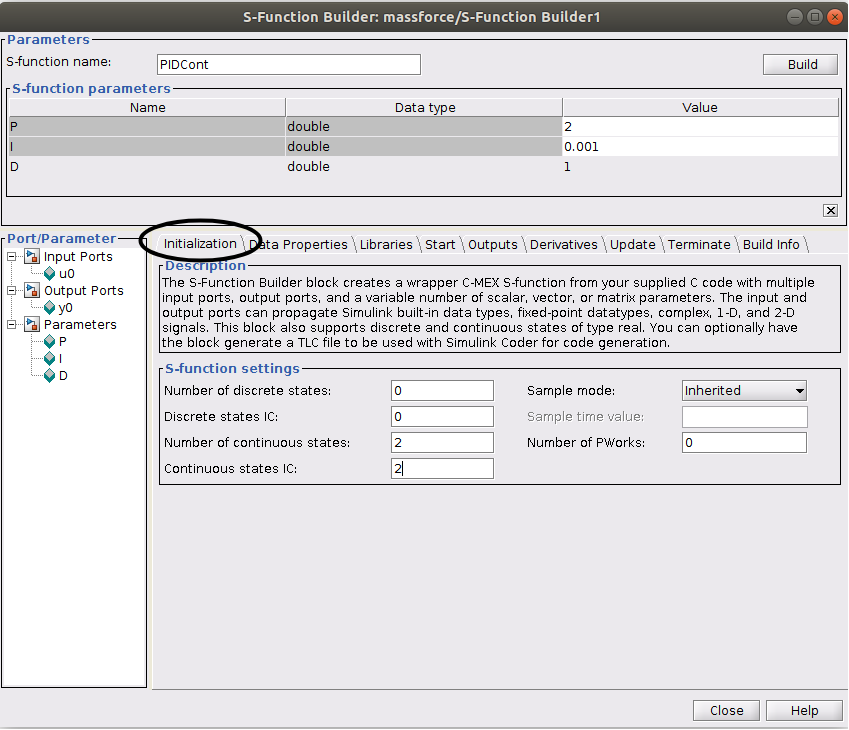
\includegraphics[width=0.8\textwidth]{Initialize.png}
    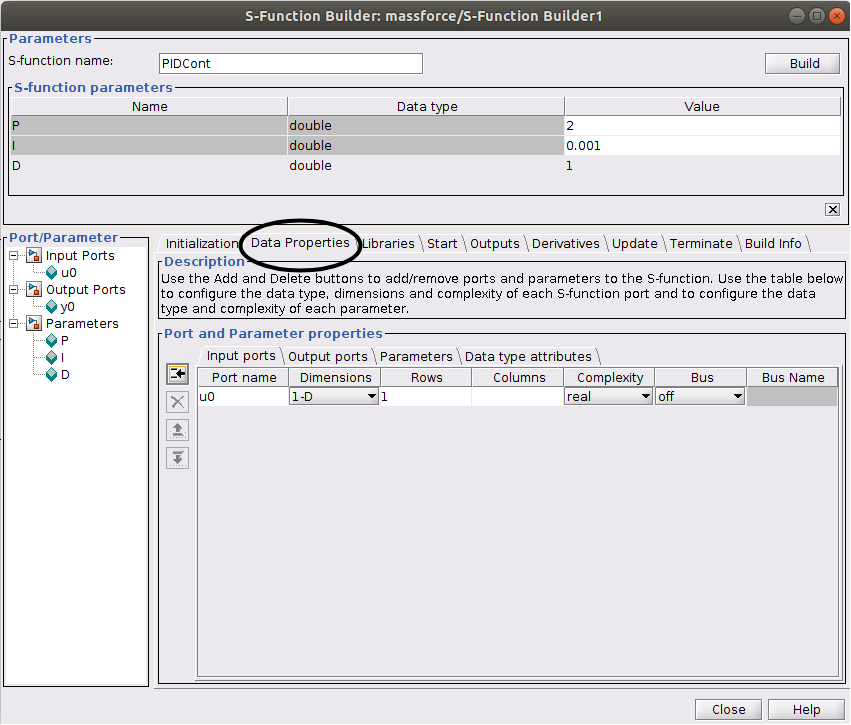
\includegraphics[width=0.8\textwidth]{Datatab2.png}
    \caption{First is the Initialization tab and Second is the Data properties tab}
    \label{fig:ex1}
\end{figure}
\begin{figure}[H]
    \centering
    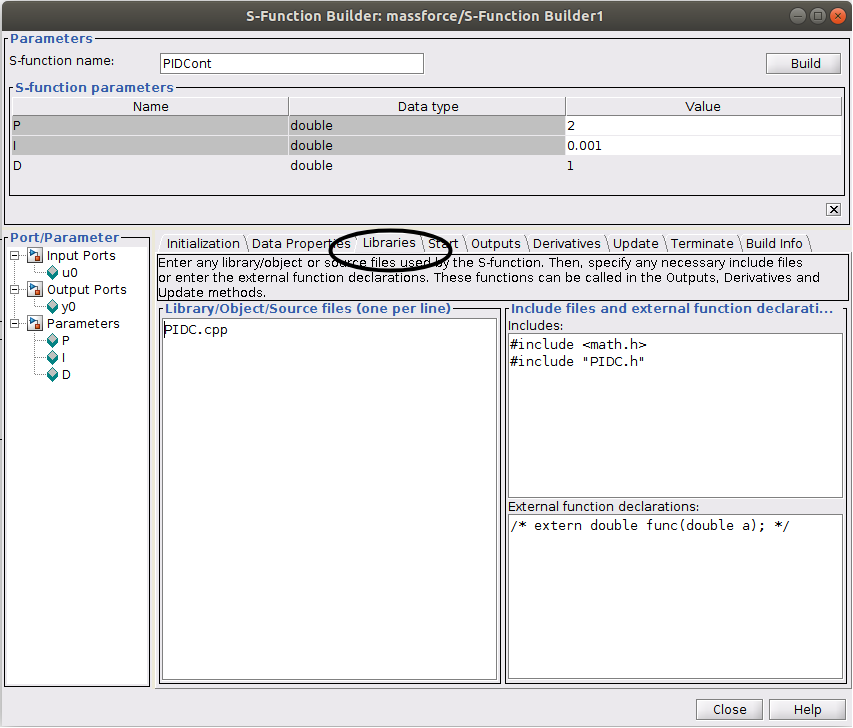
\includegraphics[width=0.8\textwidth]{librariestab3.png}
    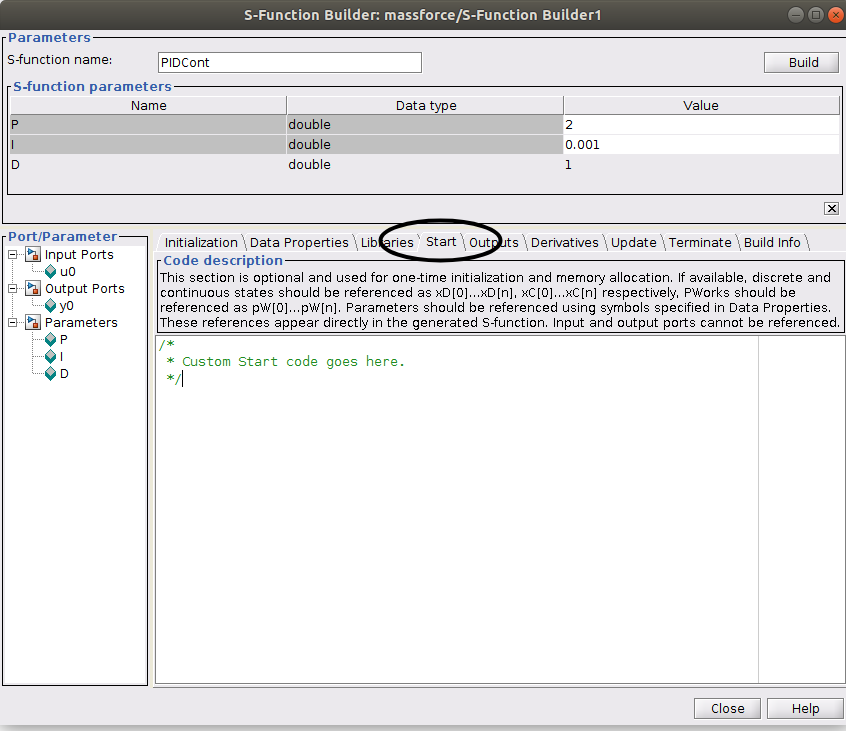
\includegraphics[width=0.8\textwidth]{starttab4.png}
    \caption{Libraries and Start tab.}
    \label{fig:ex2}
\end{figure}
\begin{figure}[H]
    \centering
    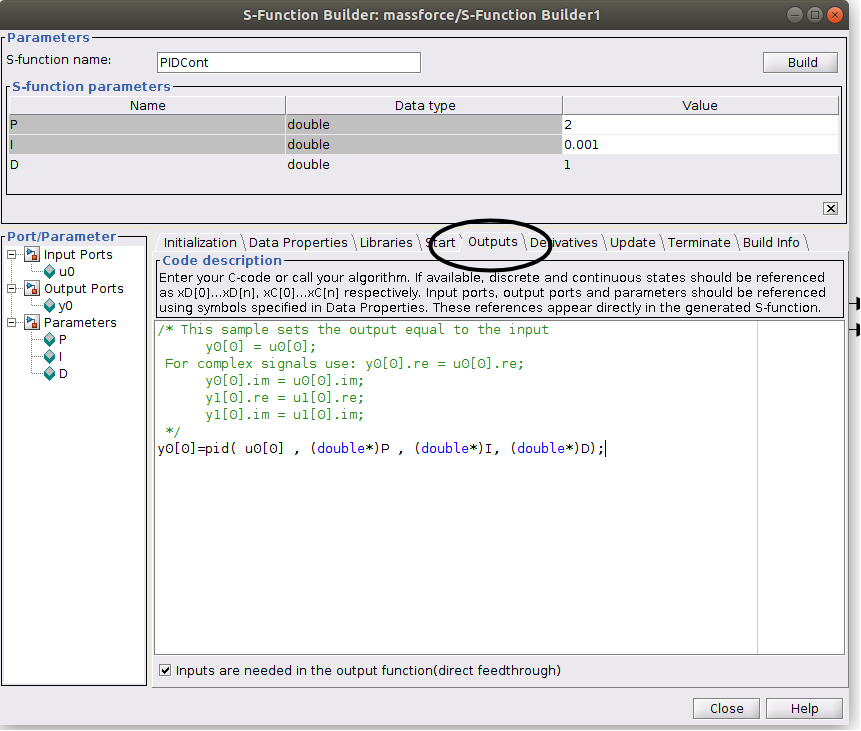
\includegraphics[width=0.8\textwidth]{outputtab5.png}
    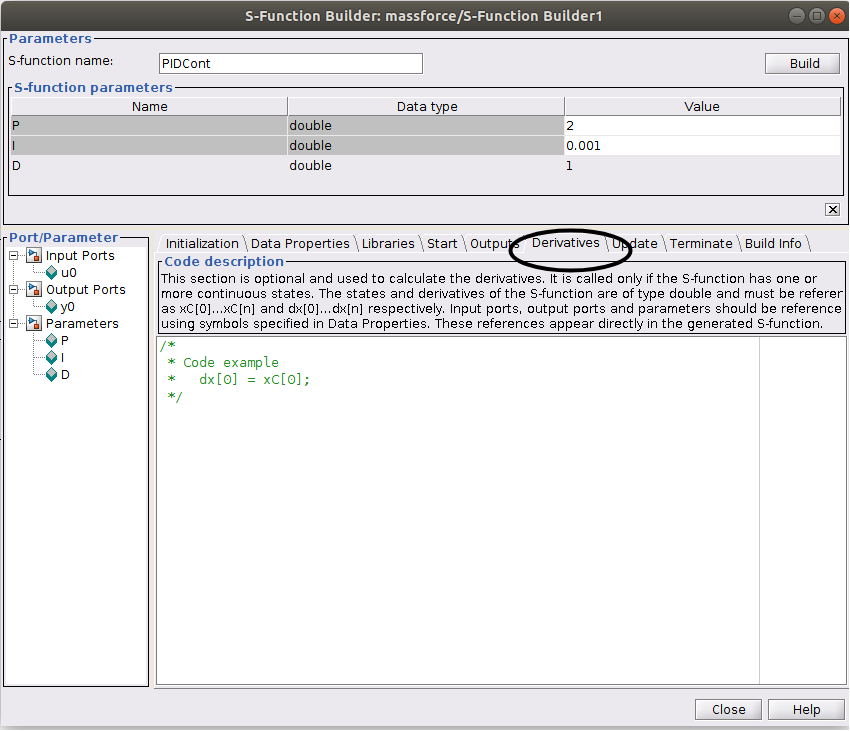
\includegraphics[width=0.8\textwidth]{derivativestab6.png}
    \caption{Output and Derivative tab}
    \label{fig:ex3}
\end{figure}
\begin{figure}[H]
    \centering
    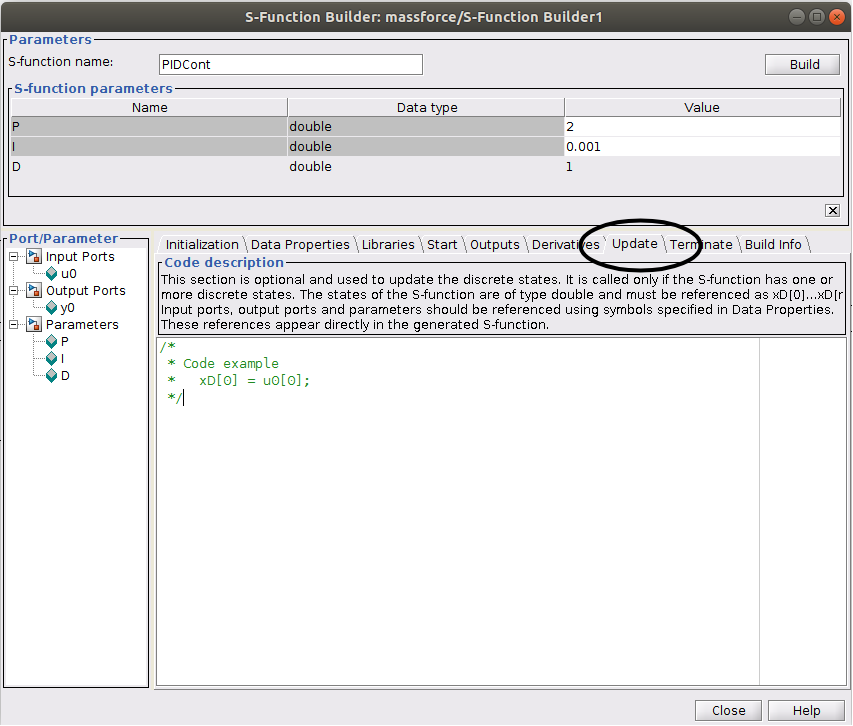
\includegraphics[width=0.8\textwidth]{updatetab7.png}
    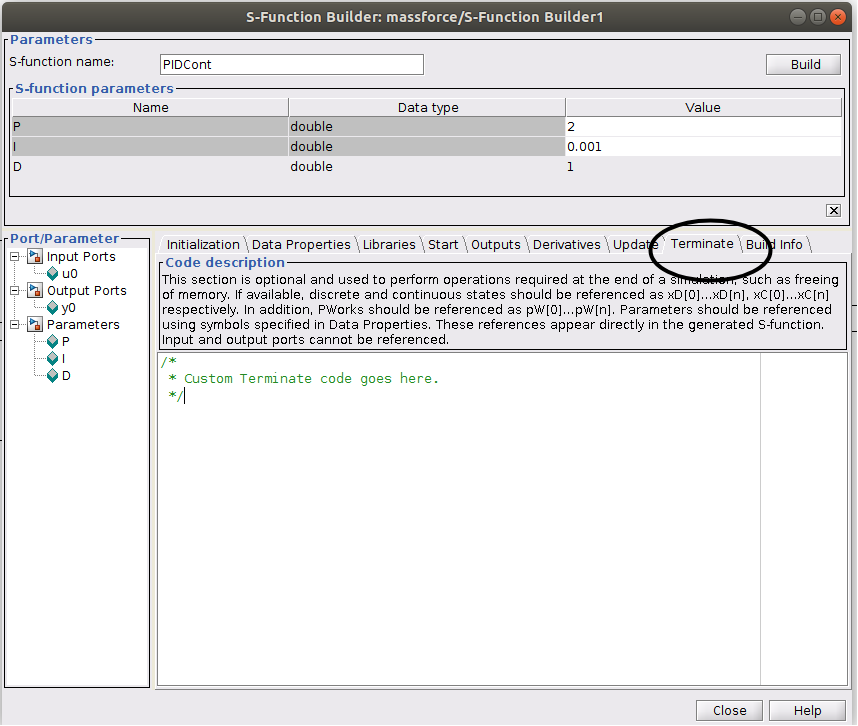
\includegraphics[width=0.8\textwidth]{terminatetab8.png}
    \caption{Update and Terminate tab}
    \label{fig:my_label}
\end{figure}[H]
\begin{figure}
    \centering
    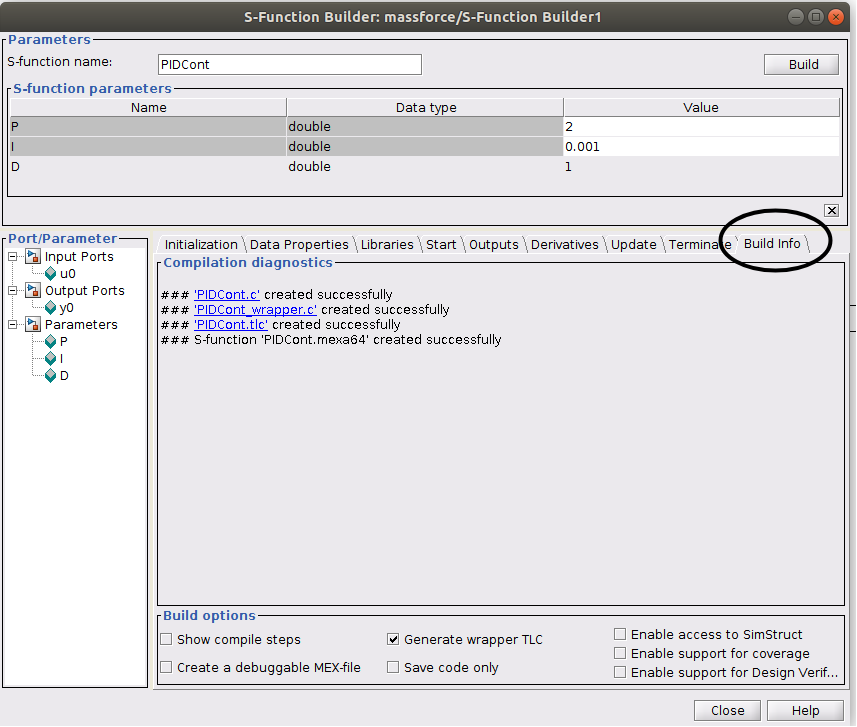
\includegraphics[width=0.8\textwidth]{builddtab9.png}
    \caption{Build Info tab}
    \label{fig:my_label}
\end{figure}
\newpage
\subsection*{Example of the wrapper.c and function.c files created my Matlab.}
\subsubsection*{Wrapper.c file}
\begin{figure}[H]
    \centering
    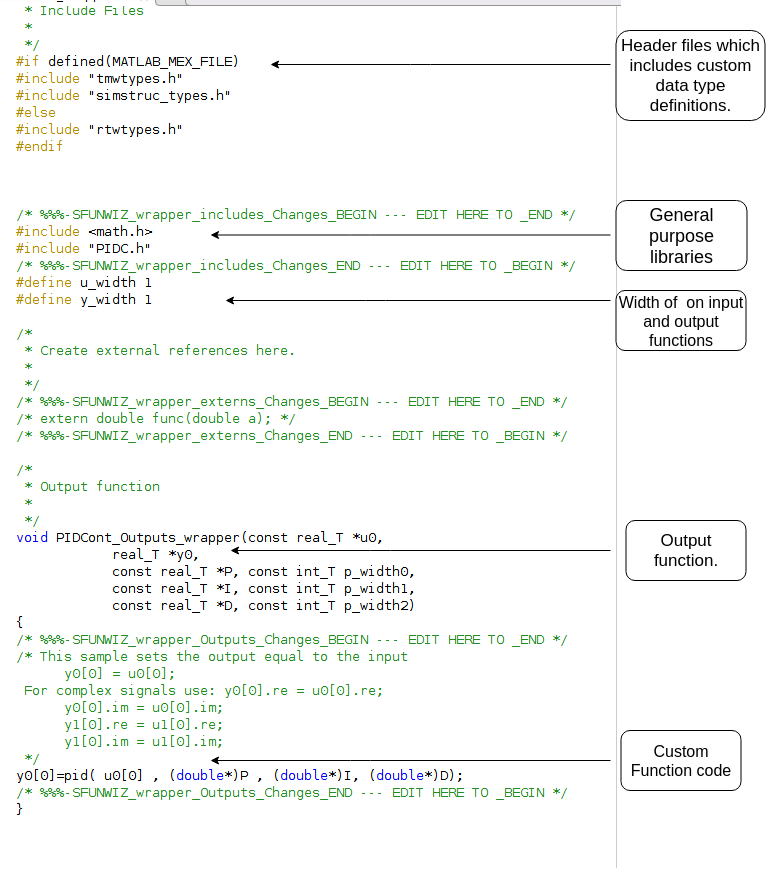
\includegraphics[width=\textwidth]{wrapper.png}
    \label{fig:my_label}
\end{figure}
\subsection*{C file}
\begin{figure}[H]
    \centering
    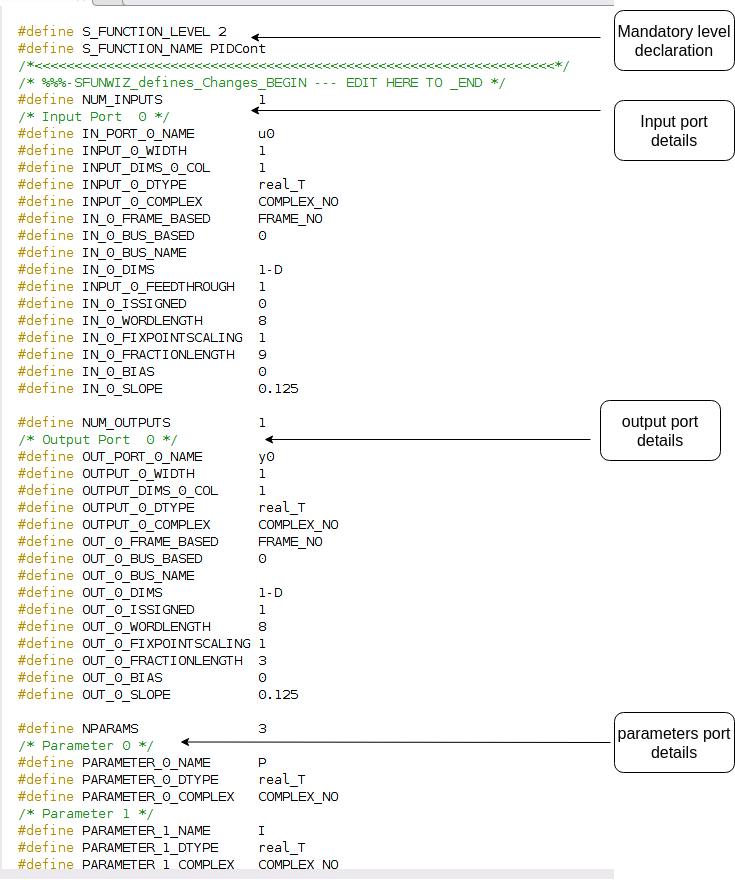
\includegraphics[width=\textwidth]{Cfile(1).png}
    \label{fig:my_label}
\end{figure}
\begin{figure}[H]
    \centering
    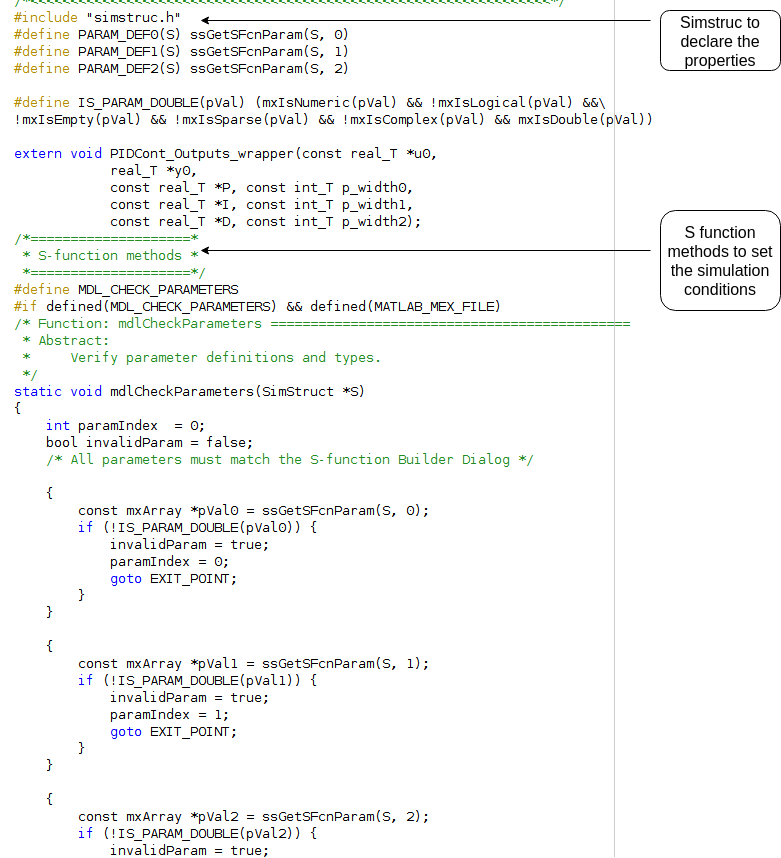
\includegraphics[width=\textwidth]{Cfile(2).png}
    \label{fig:my_label}
\end{figure}
\begin{figure}[H]
    \centering
    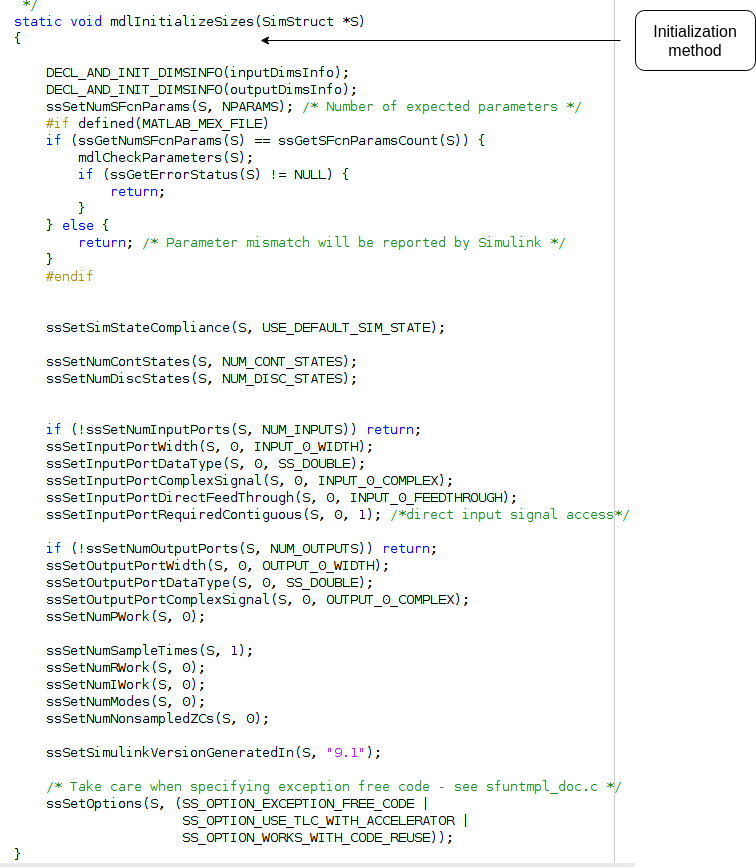
\includegraphics[width=\textwidth]{Cfile(3).png}
    \label{fig:my_label}
\end{figure}
\begin{figure}[H]
    \centering
    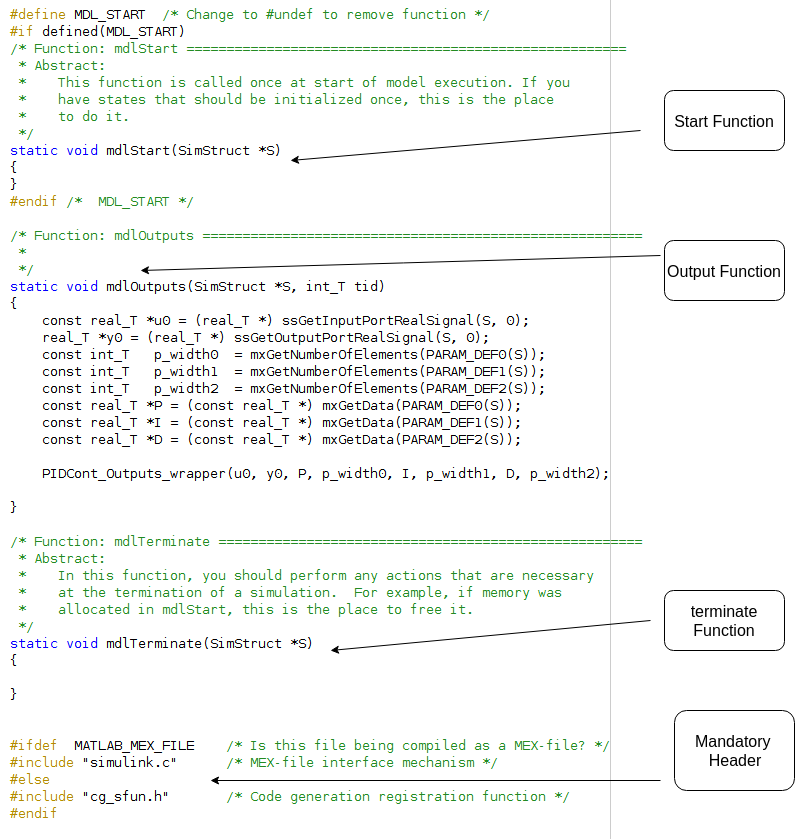
\includegraphics[width=\textwidth]{Cfile(4).png}
    \label{fig:my_label}
\end{figure}




\end{document}
